\begin{figure}[ht!]
    \centering
    % % \includegraphics[width=\textwidth,keepaspectratio]{images/compiled_figures/MRS_Sim_Figure_10_Voigt_Broadening_samples.eps}
    % \begin{tabular}[c]{ccc}
    % \begin{subfigure}[c]{0.31\textwidth}
    %     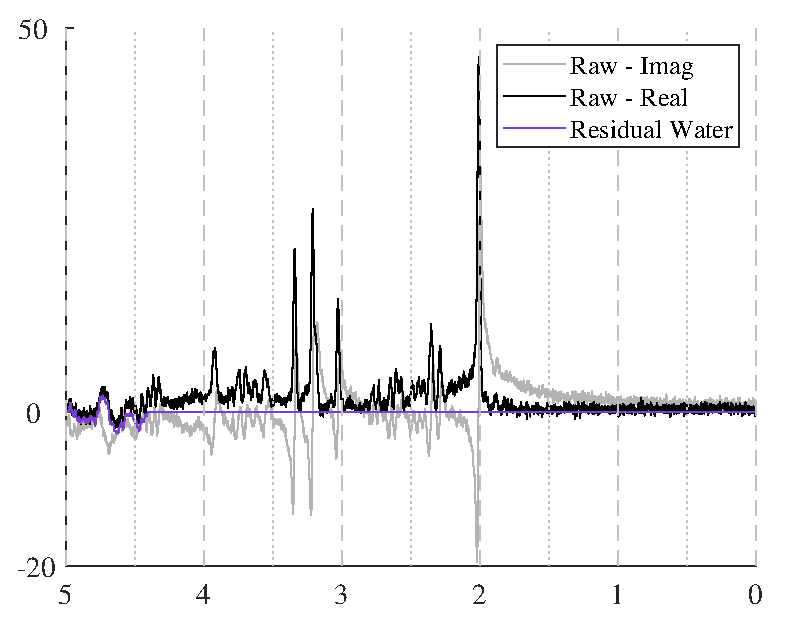
\includegraphics[width=0.93\textwidth]{images/samples_by_artifact/30ms_artifact_samples_voigt_1.eps}
    %     \caption{${T_2}^* \times 0.10$ and $G=20$Hz}
    %     \vspace{3pt}
    % \end{subfigure}&
    % \begin{subfigure}[c]{0.31\textwidth}
    %     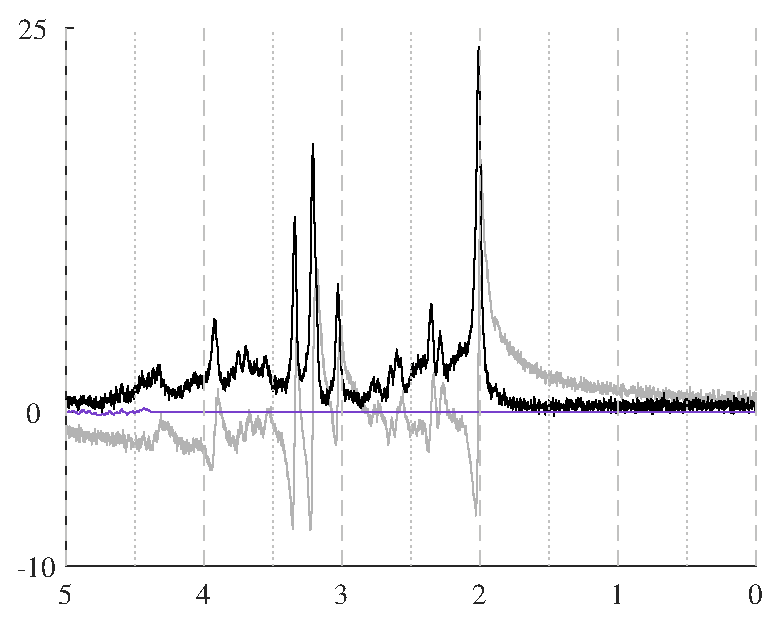
\includegraphics[width=0.93\textwidth]{images/samples_by_artifact/30ms_artifact_samples_voigt_2.eps}
    %     \caption{${T_2}^* \times 1.00$ and $G=20$Hz}
    %     \vspace{3pt}
    % \end{subfigure}&
    % \begin{subfigure}[c]{0.31\textwidth}
    %     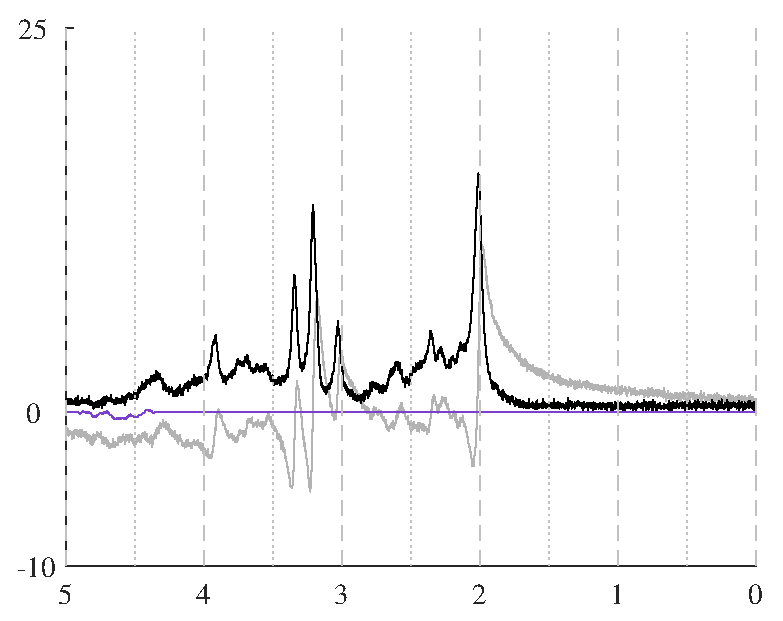
\includegraphics[width=0.93\textwidth]{images/samples_by_artifact/30ms_artifact_samples_voigt_3.eps}
    %     \caption{${T_2}^* \times 2.00$ and $G=20$Hz}
    %     \vspace{3pt}
    % \end{subfigure}\\
    % \begin{subfigure}[c]{0.31\textwidth}
    %     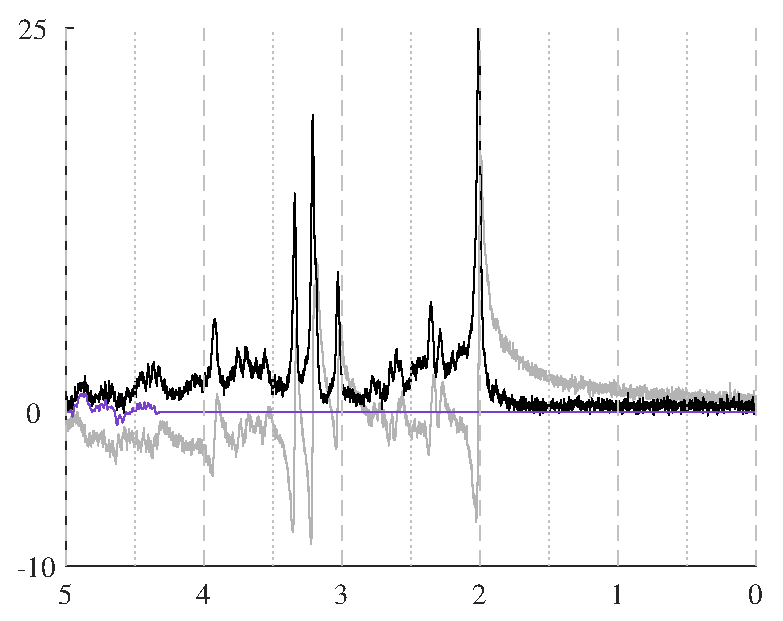
\includegraphics[width=0.93\textwidth]{images/samples_by_artifact/30ms_artifact_samples_voigt_4.eps}
    %     \caption{${T_2}^* \times 1.00$ and $G=10$Hz}
    %     \vspace{3pt}
    % \end{subfigure}&
    % \begin{subfigure}[c]{0.31\textwidth}
    %     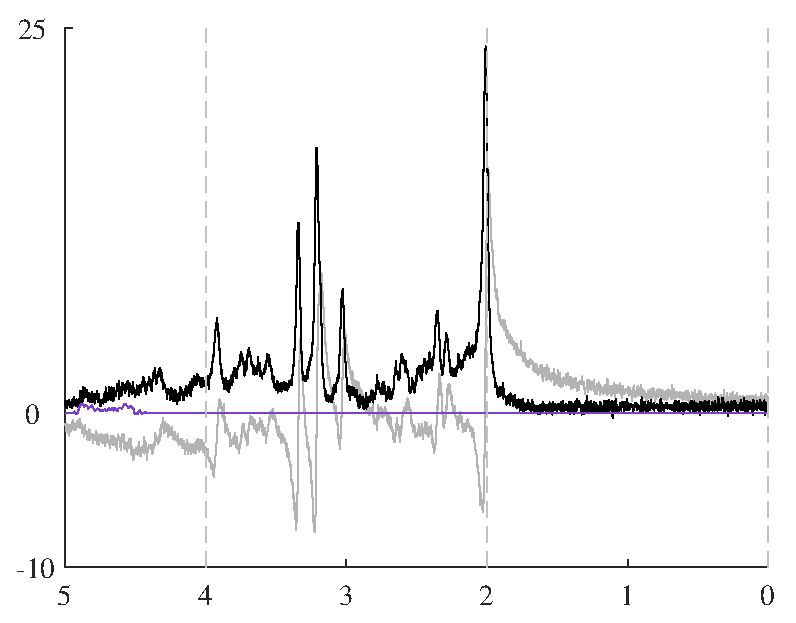
\includegraphics[width=0.93\textwidth]{images/samples_by_artifact/30ms_artifact_samples_voigt_5.eps}
    %     \caption{${T_2}^* \times 1.00$ and $G=20$Hz}
    %     \vspace{3pt}
    % \end{subfigure}&%
    % \begin{subfigure}[c]{0.31\textwidth}
    %     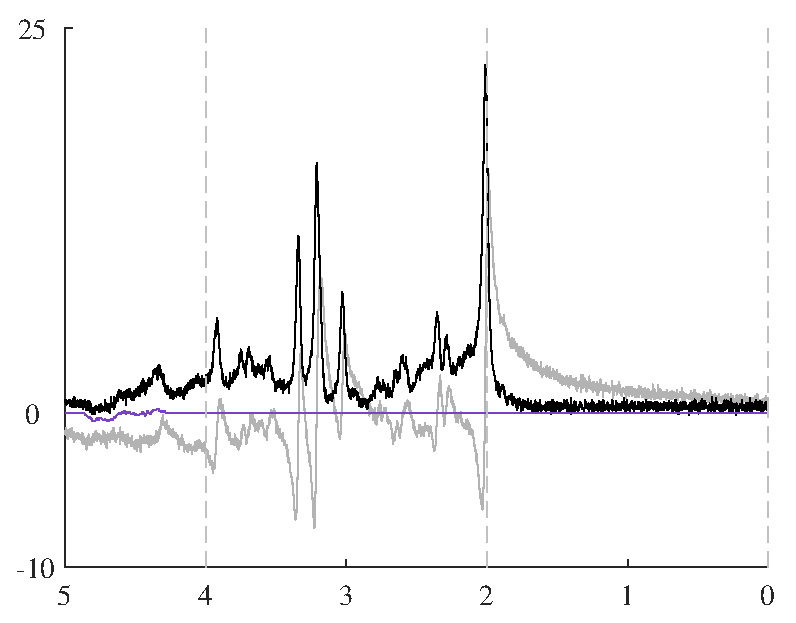
\includegraphics[width=0.93\textwidth]{images/samples_by_artifact/30ms_artifact_samples_voigt_6.eps}
    %     \caption{${T_2}^* \times 1.00$ and $G=30$Hz}
    %     \vspace{3pt}
    % \end{subfigure}\\
    % \end{tabular}
    \includegraphics[width=\textwidth,keepaspectratio]{images/compiled_figures/MRS_Sim_Figure_10_Voigt_Broadening_samples.png}
    \caption{Theses samples explore the effects of lorentzian and gaussian broadening on the Voigt lineshape. The spectral SNR = 15. No phase offsets, eddy currents, or baselines were included. The top row varies the lorentzian broadening with a fixed gaussian value where the bottom row fixes the lorentzian broadening values and varies the gaussian.}
    \label{fig:30ms samples voigt}
\end{figure}

